%!TEX program = xelatex
\documentclass[12pt, a4paper, oneside]{ctexart}
\usepackage[utf8]{inputenc}
\usepackage{ctex} %导入中文包
\usepackage{listings}
\usepackage{fontspec}
\usepackage{geometry} %设置页边距的包
\usepackage{listings}
\usepackage{xcolor} 

\usepackage{graphicx}
\usepackage{float}


\title{\fontsize{70}{30}\selectfont  ACM 算法    爆哥 \& Buns\_out  合订模板} 
\author{无敌爆哥 \& Buns\_out} 
\date{\today} 

\geometry{left=2.5cm,right=2cm,top=2.54cm,bottom=2.54cm} %设置书籍的页边距
\definecolor{mygray}{rgb}{0.97,0.97,0.97}%定制颜色

\setsansfont{Monaco} 
\setmainfont{Monaco}


%对于lstset排版
\lstset{
tabsize=4,
	breaklines, 					% 自动将长的代码行换行排版
	backgroundcolor = \color{white},     			 % 背景色:淡黄
	numbers=left, 									% 行号在左侧显示
	numberstyle= \small, 								% 行号字体
	keywordstyle= \color{ red!70},						 % 关键字颜色
	commentstyle= \color{red!50!green!50!blue!50}, 		% 注释颜色
	rulesepcolor= \color{ red!20!green!20!blue!20} ,
	frame=single,                               % 设置代码框形式
	escapeinside=``,									 % 英文分号中可写入中文
	xleftmargin=2em,xrightmargin=2em, aboveskip=1em,
	framexleftmargin=2em
} 


\begin{document} 

\maketitle
\thispagestyle{empty}
\centering
% 
\includegraphics[scale=0.55]{pic.jpg}


\newpage
\tableofcontents 
\thispagestyle{empty}
\lstset{language=C++}


\newpage 
\section{爆哥滴}
\subsection{拓展卢卡斯} 
mod不需要为质数
求阶乘部分可以适当的用记忆化
\begin{lstlisting}
ll fac(ll n,int p,int mod){
    if(!n) return 1;
    ll res=1;
    for(int i=2;i<=mod;i++){
        if(i%p) res=res*i%mod;
    }
    res=ksm(res,n/mod,mod);
    for(int i=2;i<=n%mod;i++){
        if(i%p) res=res*i%mod;
    }
    return res*fac(n/p,p,mod)%mod;
}
ll Inv(ll a,ll mod){
    ll x,y;
    exgcd(a,mod,x,y);
    return (x+mod)%mod;
}
ll C(ll n,ll m,int p,int mod){
    ll d=fac(n,p,mod),d1=fac(m,p,mod),d2=fac(n-m,p,mod);
    ll k=0;
    for(ll i=n;i;i/=p){
        k+=i/p;
    }
    for(ll i=m;i;i/=p){
        k-=i/p;
    }
    for(ll i=n-m;i;i/=p){
        k-=i/p;
    }
    return d*Inv(d1,mod)%mod*Inv(d2,mod)%mod*ksm(p,k,mod)%mod;
}
ll exlucas(ll n,ll m,int p){
    if(n<0||m<0||n<m) return 0;
    int x=p;
    tp=0;
    for(int i=2;1ll*i*i<=x;i++){
        if(x%i==0){
            int t=1;
            while(x%i==0){
                x/=i;t*=i;
            }
            ++tp;
            r[tp]=C(n,m,i,t);
            md[tp]=t;
        }
    }
    if(x>1) {
        ++tp;
        r[tp]=C(n,m,x,x),md[tp]=x;
    }
    return CRT();
}
\end{lstlisting}

\newpage 
\subsection{复数} 
\begin{lstlisting}
struct complex_{
	double a,b;
	complex_(){a=0;b=0;}
	complex_(double _a,double _b){a=_a;b=_b;}
	complex_ operator +(const complex_ &w)const{
		return complex_(a+w.a,b+w.b);
	}
	complex_ operator -(const complex_ &w)const{
		return complex_(a-w.a,b-w.b);
	}
	complex_ operator *(const complex_ &w)const{
		return complex_(a*w.a-b*w.b,a*w.b+b*w.a);
	}
	complex_ operator /(const complex_ &w)const{
		return complex_(a*w.a+b*w.b,b*w.a-a*w.b)/(w.a*w.a+w.b*w.b);
	}
	complex_ operator /(const double w){
        return complex_(a/w,b/w);
    }
};
\end{lstlisting}

\newpage 
\subsection{数据范围对应最大因子与质因子} 
\centering 
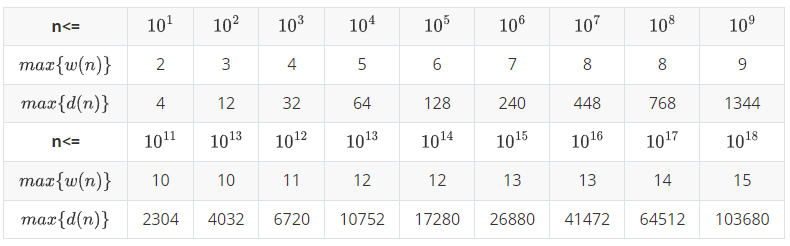
\includegraphics[scale=0.85]{bg.png}
\flushleft

\newpage 
\subsection{三元环计数} 
\begin{lstlisting}
for(int i=1;i<=m;i++){
        in[p[i].v]++;
        in[p[i].u]++;
    }
    for(int i=1;i<=m;i++){
        int x=p[i].v,y=p[i].u;
        if(in[x]>in[y]) swap(x,y);
        else if(in[x]==in[y]&&x>y) swap(x,y);
        v[x].push_back(y);
    }
    int ans=0;
    for(int i=1;i<=n;i++){
        for(int k:v[i]) up[k]=i;
        for(int j:v[i]){
            for(int k:v[j]){
                ans+=(up[k]==i);
            }
        }
    }
\end{lstlisting}

\newpage
\section{Buns\_out滴}
\subsection{Lyndon分解} 
\begin{lstlisting}
/*
将S分成若干个部分S=S1S2S3..Sm 每个串都是 Lyndon Word
一个字符串 s 是一个 Lyndon Word 表示 s 是其所有后缀中的最小者。
*/
vector<string> duval(string const &s) {
	int n = s.size(), i = 0;
	vector<string> fac;
	while (i < n) {
		int j = i + 1, k = i;
		while (j < n && s[k] <= s[j]) {
			if (s[k] < s[j]) k = i;
			else k++;
			j++;
		}
		while (i <= k) {
			fac.push_back(s.substr(i, j - k));
			i += j - k;
		}
	}
	return fac;
}
// duval_algorithm
vector<int> duval2(string const &s) {
	int n = s.size(), i = 0;
	vector<int> fac;
	while (i < n) {
		int j = i + 1, k = i;
		while (j < n && s[k] <= s[j]) {
			if (s[k] < s[j])k = i;
			else k++;
			j++;
		}
		while (i <= k) {
			i += j - k;
			fac.push_back(i);
		}
	}
	return fac;
}
void solve()
{
	string s;
	cin >> s;
	auto v = duval2(s);

	for (auto i : v) {
		cout << i << " ";
	}
}
\end{lstlisting}

\newpage
\subsection{Linux对拍} 
\begin{lstlisting}
int main(){
	while(1){
		printf("The result of No. %d Case is:  ",++cases);
		system("./data");
		system("./BF");
		system("./test");
		if(system("diff BF.out test.out")){
			puts("Wrong Answer\n");
			return 0;
		}
		puts("Accepted");
	}
	return 0;
}
\end{lstlisting}


\newpage
\subsection{在线查询回文子串数量} 
\begin{lstlisting}
/*
1:在字符串 s 的末尾添加一个字符串
2:在字符串 s 的前端添加一个字符串的 反序
3:查询字符串 s 的所有非空回文子串的数量
*/


struct PAM {
	char s[maxn];
	int ptrf, ptrb;
    int node, len[maxn + 5], fail[maxn + 5], ch[maxn + 5][26];
    int rlas, llas, dep[maxn + 5];

    PAM() { node = rlas = llas = 1, len[1] = -1, fail[0] = 1; }
    void set(int _x,int _y){
    	ptrf=_x;
    	ptrb=_y;
    }

    inline int push_front( char c ) {
        s[--ptrf] = c, c -= 'a'; int p = llas;
        for ( ; s[ptrf + len[p] + 1] != s[ptrf]; p = fail[p] );
        if ( !ch[p][c] ) {
            len[++node] = len[p] + 2; int q = fail[p];
            for ( ; s[ptrf + len[q] + 1] != s[ptrf]; q = fail[q] );
            dep[node] = dep[fail[node] = ch[q][c]] + 1, ch[p][c] = node;
        }
        llas = ch[p][c];
        if ( len[llas] == ptrb - ptrf + 1 ) rlas = llas;
        return dep[llas];
    }

    inline int push_back( char c ) {
        s[++ptrb] = c, c -= 'a'; int p = rlas;
        for ( ; s[ptrb - len[p] - 1] != s[ptrb]; p = fail[p] );
        if ( !ch[p][c] ) {
            len[++node] = len[p] + 2; int q = fail[p];
            for ( ; s[ptrb - len[q] - 1] != s[ptrb]; q = fail[q] );
            dep[node] = dep[fail[node] = ch[q][c]] + 1, ch[p][c] = node;
        }
        rlas = ch[p][c];
        if ( len[rlas] == ptrb - ptrf + 1 ) llas = rlas;
        return dep[rlas];
    }
}pam;
string str;
ll ans=0;
int q;
void solve()
{
	pam.set(3e5+1,3e5);
	cin>>str;
	for(auto i:str)
		ans+=pam.push_back(i);
	cin>>q;
	while(q--)
	{
		int op;
		cin>>op;
		if(op==1)
		{
			cin>>str;
			for(auto i:str)
				ans+=pam.push_back(i);
		}
		else if(op==2)
		{
			cin>>str;
			for(auto i:str)
				ans+=pam.push_front(i);
		}
		else cout<<ans<<endl;
	}
}
\end{lstlisting}




\end{document}